\chapter{\textbf{Delay Estimation framework}}
\label{chap:estimation}
As already mentioned before, to decide on a solution (super arm), we need first to gain estimation for each individual's arms. In our problem, we assume that by selecting a super arm, we are able to get an estimation of every single arm in it (i.e: computing delay and link delay) and update the estimated values accordingly. 
In this chapter, we present our design of a time-stamped based estimation framework to measure the delay in the network, which we implement and apply for each Mininet-WiFi experiment conducted in chapter \ref{chapter: Mininet-wifi Experiments}. 

%\subsection{Related work}
%Probing techniques have been well studied in the literature. We introduce two approaches: \cite{article, alizadeh2014conga} propose two different methods of probing in order to get the link information and use them in routing and load balancing, respectively.
%
%In \cite{alizadeh2014conga}, the authors present Conga, which focuses on the measurement of a link load. The idea of this method to measure a link between two nodes is to send packets and create a feedback loop between the sender and receiver to populate the metrics through the link. To store and estimate the metrics, they use DRE (discounted rate estimator), which maintains a register $X$, that is incremented for each packet sent over the link by the packet size in bytes and is decremented periodically with a multiplicative factor $\alpha$ between 0 and 1: $X = X\times(1-\alpha)$. 
%The metric that needs to be measured in their case is congestion between two nodes.
%
%Authors in HyMAB \cite{article}
%on the other hand, focus on the strategy of finding optimal multi-path for a single flow in routing problem in order to get an optimal throughput. The proposed algorithm HyMAB, treats each multi-path as arms. Each time it chooses one multi-path to probe and get a reward. The arm is chosen based on a multi-arm bandit strategy that is introduced in \cite{auer2002finite}.
%
%After an arm is chosen, which means the multi-path is given, they compute an optimal rate on this path by solving a max rate linear problem.

\section{Time stamp in SFC placement}
Now we present our proposed time-stamp based estimation framework in SFC placement to measure the processing delays on each computing node and the transmission delay on each link. %Estimation of these two metrics will be stored in a SFC capacity vector (denoted by $E$) that returns to the user along with the SFC response.
To estimate the delays in the network, we time-stamp\cite{} one packet and tag it along with the packets we send for each SFC request while keeping track of the time. The estimation is consist of two parts:

1) \textbf{An initial estimation of the whole network.} The user first sends a request to each computing node. Upon receiving the request, the server will each send packets to the other servers and time stamp them. After receiving all the returned packets, the server parses the timestamps in them, calculates the delays, and sends that information back to the user. The user collects all the delay estimations from the servers and saves them as a initial estimation required in the CMAB algorithm.

2) \textbf{Estimation of delays on the nodes and links that have been selected for placeing SFCs.} Like the initial estimation, we also timestamp the packets we send in each SFC request. After the packet is returned from the SFC, the user parses the timestamps and calculate the delays on the SFC. Those estimations will then be used to update the initial estimation according to algorithm~\ref{alg:cccpa}.
We consider a SFC with three different services in this section as an example. The packet format of the packet that's used for estimation is shown in figure \ref{fig:estimation packet format}. Each server on the path appends the timestamps to the packet as the packet traverses. Depending on the length of SFC, say $l$, each estimation packet would occupy $(l+1)*18$ bytes of payload to store all the timestamps because each time stamps takes 18 bytes to store in our implementation.


% \begin{itemize}

%     % \item \textbf{$nid_i (2 bytes)$}: this field is used by the nodes along the path to store the node id of the $i$th node in the SFC.
%     \item \texbf{$\Lambda_i(4bytes)$} : this field is used to store the size of SFC packets
%     \item \textbf{$t_i(4bytes)$}: link capacity, this field is used to store the time stamp.

%     % \item \textbf{DT}: Delay Table, This is a M-M table that stores the transmission delays in the networks at time slot t, specifically for a node i, $T^t_i = [g^t_{i,1}, g^t_{i, 2}, ..., g^t_{i, M}]$, this table will be maintained by destination node based on index: SN and DN, one transmission delay metric will be inserted in this table after destination node receive the probe packet and calculate a delay.    

% \end{itemize}
\begin{figure}
	\centering
	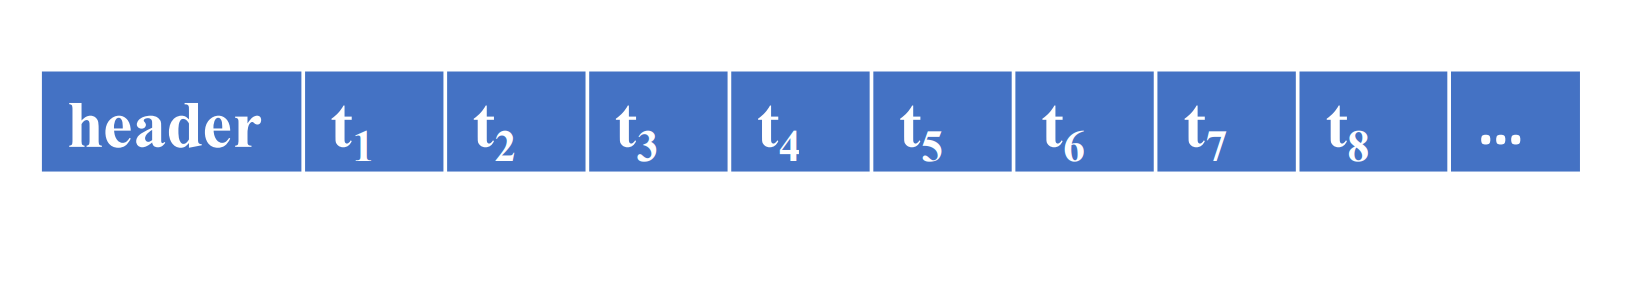
\includegraphics[width=0.9\linewidth]{figs/packetformat.PNG}
	\caption{Estimation packet format}
	\label{fig:estimation packet format}
\end{figure}
% \subsubsection{Delay feedback}
% We use a feedback loop between the source node and the destination node for us to gain estimations for Computing capacity vector and transmission delay table. The probing process is described as follow:
% \begin{enumerate}
%     \item The source node first sends the probe packet to MEC network with the $nid_1$ field set to its node id and $c_i$ set to its computing capacity. 
%     \item As the packet routing through the MEC, each nodes it passes will calculate the link capacity from the last node before it process the packets and add it to f field, it also calculates it own computing capacity and insert it into $C^t$ vector in CC field.
%     \item When the packet is received at the destination node, it will add its transmission delay from last node to the TD field which will be the delay estimation from source node to destination node. Then it will add its computing capacity to the CC field and prepare for piggyback.
%     \item when a packet is sent in the reverse direction, the aggregated delay metric will be inserted to the delay table based on the source node id in SN field and destination node id.
%     \item Finally, the source node received and parse the piggyback packet and get a partial estimation of capacity vector and delay table.
% \end{enumerate}

%\subsection{SFC feedback}
%\subsubsection{SFC-to-user feedback loop}
%In our user-based SFC problem, we use a SFC-to-user feedback loop to obtain the network information. Explicitly we assume that probing process is within the SFC process, that is, when the SFC request is roaming through the VNFs (virtual network functions), the estimation packet will also be passed on the nodes that has the VNFs placed on along with the SFC packets. In the end of a time slot, the user will not only receive a SFC response but also an updated estimation vector, this process is illustrated in figure 5.
%\begin{figure}
%    \centering
%   \includegraphics[width=0.7\textwidth]{probingservicechain.PNG}
%  \caption{Probing in SFC placement}
% \label{fig:my_label}
%\end{figure}
\section{Time-stamped delay estimation example}
We consider a scenario that the VNFs are placed on node A, B, C at the moment and that the user is connected to node D, as shown in figure~\ref{fig:timestampExample}. The SFC request from a mobile user will be time-stamped and saved as a vector as we defined before, as the request is handled along the chain, each processing node will time stamp the packet when: 1) When it receives a packet, 2) After it is done processing. The probing process is described as follow:

1) User generates SFC request packets with size $\lambda_i$ bytes for each service $i$, while inserting the current time to $t_1$ in the last packet.

2) Node A receives the request first in the SFC. Upon receiving the last packet, it updates the packet by inserting its current time to $t_2$ and starts processing the packets. When the processing is done, node A inserts the current time $t_3$ to the same packet. Then it sets the destination to node B as the next service handler and forwards all the packets.

3) Node B process the second requested task and inserts timestamps $t_4$, $t_5$ before and afterward the task, respectively. Then it sets the destination to C and forwards the packets.

4) Node C processes the last request. It repeats the time-stamping ($t_6$, $t_7$) and sends a SFC response along with a packet that stores all the timestamps in order.

5) the user will then get a response for their services and a list of timestamps while recording the current time $t_8$ upon receiving. Based on the timestamps and SFC packet sizes, the user is able to calculate the corresponding link delay and processing delay.

\begin{figure}
	\centering
	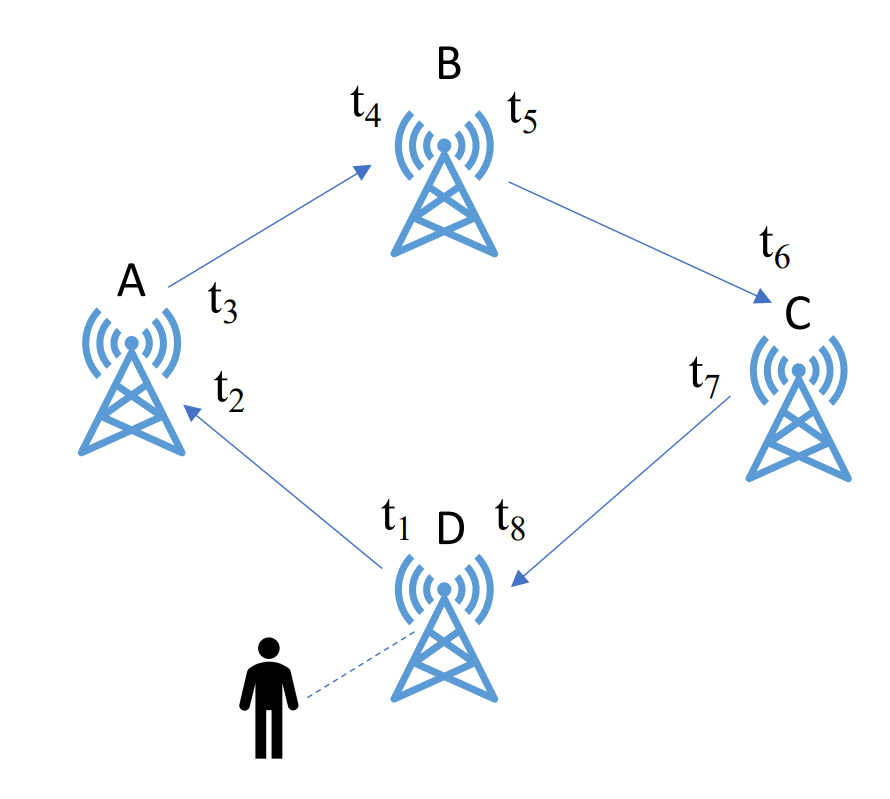
\includegraphics[width=0.9\linewidth]{figs/SFCtimestamp.PNG}
	\caption{Time stamps of SFC placement in MEC}
	\label{fig:timestampExample}
\end{figure}
When the time stamps is returned to user, they can analyze the packet and calculate the delays on the SFC path as follow:
\begin{equation}
	\label{eqn: timestampcalculation}
	\begin{aligned}
		LinkDelay_{D \rightarrow A} &= t_2 - t_1\\
		LinkDelay_{A \rightarrow B} &= t_4 - t_3\\
		LinkDelay_{B \rightarrow C} &= t_6 - t_5\\
		LinkDelay_{C \rightarrow D} &= t_8 - t_7\\
		ProcessingDelay_A           &= (t_3 - t_2)/\lambda_1\\
		ProcessingDelay_B           &= (t_5 - t_4)/\lambda_2\\
		ProcessingDelay_C           &= (t_7 - t_6)/\lambda_3\\
	\end{aligned}
\end{equation}

% We apply an adjustment term to values obtained from above to encouraging exploring for the future rounds. For each link delay and computing delay we estimate from a SFC response, we can record the times of the same element that has been updated, for element $i$, we denote the total number of times it's been updated as $T_$ and apply the following adjustment:
% \begin{equation}
% \label{eqn:adjustment}
%     \bar{\mu_i} = \hat{\mu_i} - e * \sqrt{ \frac{3\ln t}{2T_i}},
% \end{equation}
% where $t$ is the current round number, $e$ is a configurable constant.